\bob{[MAVZU] NAZARIYASI}

\subsection{Asosiy tushunchalar va farazlar}
Ushbu to’ldirgichda bir o’lchamli tekis oqim misol sifatida olinadi.
Haqiqiy ishda bu matn mavzuning ta’riflari va manbaga asoslangan izohi bilan
almashtiriladi~\cite{manba:nazariya}. $v$ --- oqim tezligi, $S$ --- kesim yuzi,
$Q$ --- hajmiy sarf. Tezlik kesim bo’ylab o’zgarmas bo’lsa,
\begin{equation}
  Q = vS.
  \label{eq:sarf}
\end{equation}
Bu yerda $v$ metr/sekundda, $S$ kvadrat metrda, $Q$ esa kub metr/sekundda
o’lchanadi. \eqref{eq:sarf} formulani qo’llashdan oldin kesimdagi tezlikning
bir jinsli ekanini asoslash kerak.

\subsection{Hisoblash munosabatlari}
Zichligi o’zgarmas oqim uchun massa sarfi quyidagicha aniqlanadi:
\begin{equation}
  \dot{m} = \rho Q.
  \label{eq:massa}
\end{equation}
Bu yerda $\rho$ --- zichlik, uning birligi $\mathrm{kg/m^3}$.
\eqref{eq:sarf} ni \eqref{eq:massa} ga qo’yib,
\begin{equation}
  \dot{m} = \rho vS
  \label{eq:umumiy}
\end{equation}
ifoda olinadi. Formulalar bob almashganda ham ketma-ket raqamlanadi.
Asosiy kattaliklar \ref{tab:kattaliklar}-jadvalda jamlangan.

\begin{table}[htbp]
  \centering
  \caption{Hisoblashdagi asosiy kattaliklar}
  \label{tab:kattaliklar}
  \begin{tabular}{|l|c|c|}
    \hline
    Kattalik & Belgisi & Birligi \\
    \hline
    Tezlik & $v$ & $\mathrm{m/s}$ \\
    Kesim yuzi & $S$ & $\mathrm{m^2}$ \\
    Hajmiy sarf & $Q$ & $\mathrm{m^3/s}$ \\
    Zichlik & $\rho$ & $\mathrm{kg/m^3}$ \\
    Massa sarfi & $\dot{m}$ & $\mathrm{kg/s}$ \\
    \hline
  \end{tabular}
\end{table}

\subsection{Grafik talqin va qo’llanish chegaralari}
\ref{fig:nazariya}-rasmda o’zgarmas kesimdagi oqim uchun hajmiy sarfning
tezlikka bog’lanishi ko’rsatilgan. Grafikdagi to’g’ri chiziq faqat yuqorida
qabul qilingan farazlar bajarilganda o’rinli. O’zgaruvchan kesim yoki notekis
tezlik taqsimoti uchun model qayta ko’rib chiqiladi.

\begin{figure}[htbp]
  \centering
  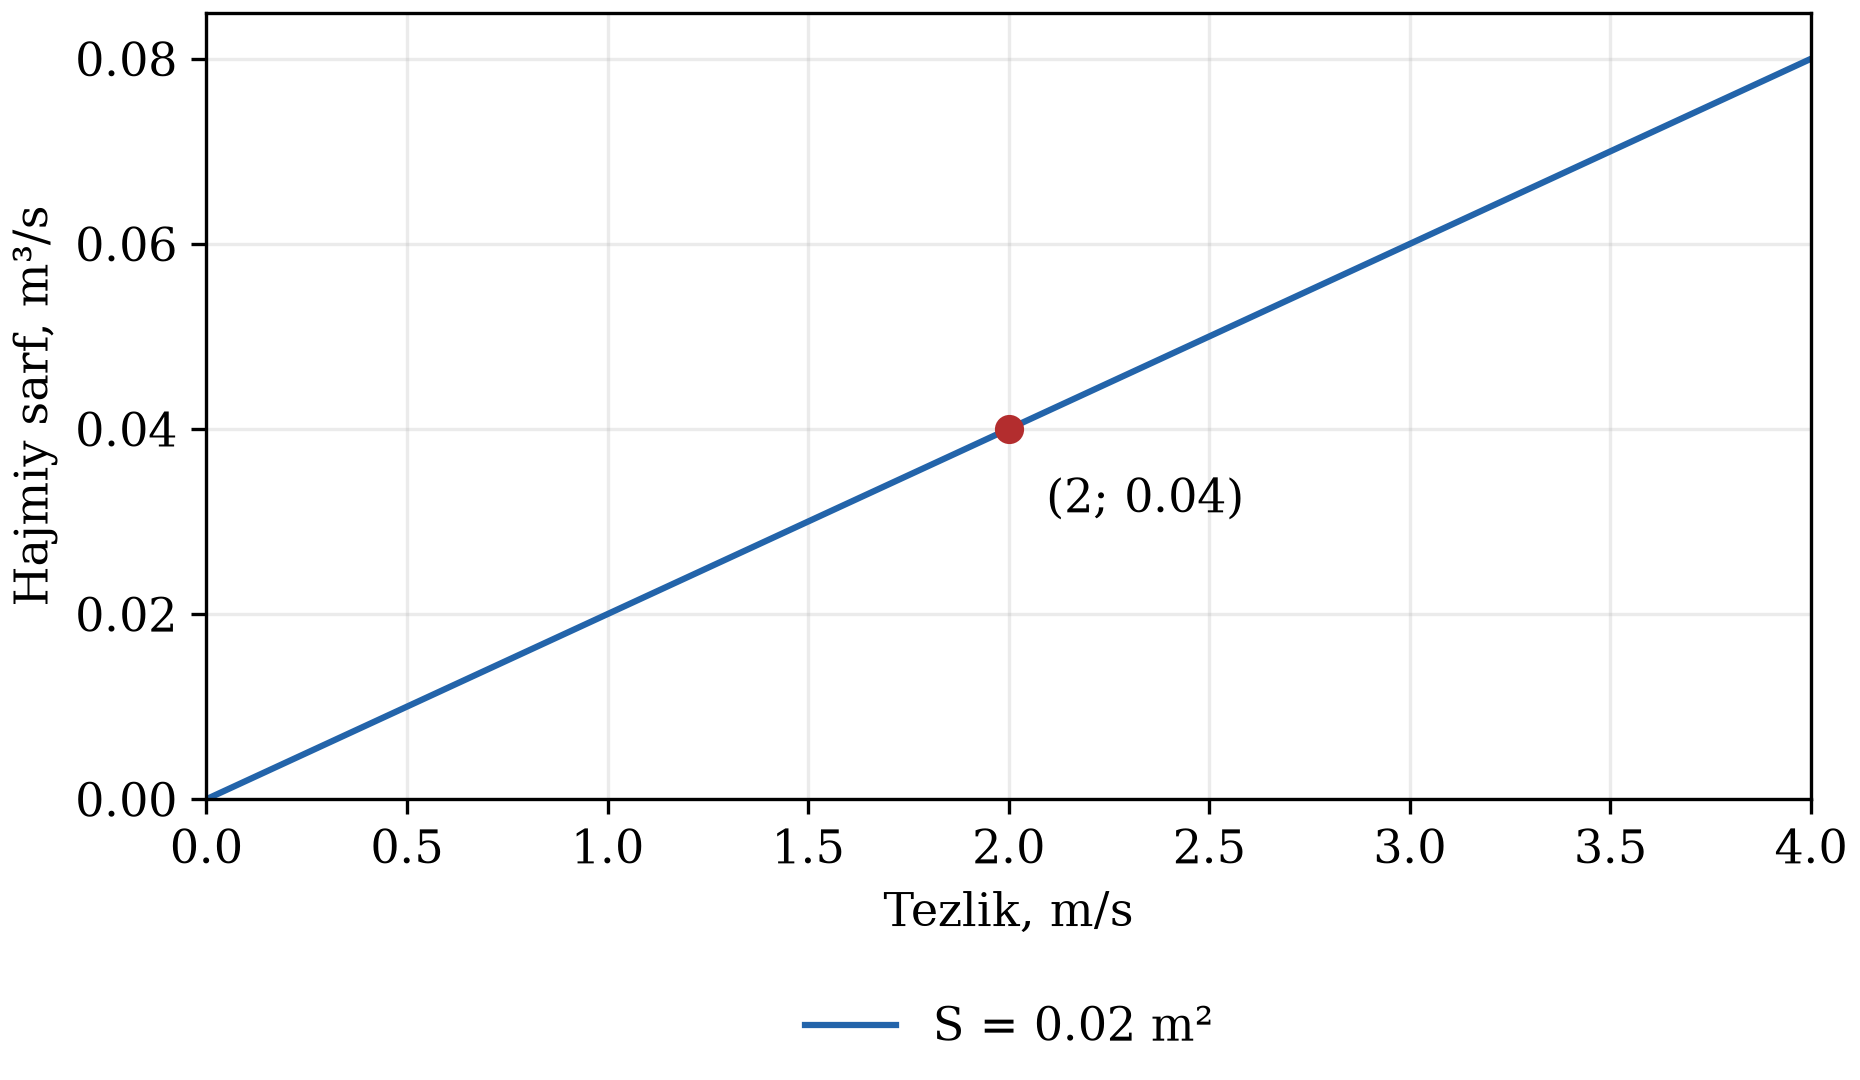
\includegraphics[width=0.70\textwidth]{namuna.png}
  \caption{O’zgarmas kesimda sarfning tezlikka bog’lanishi}
  \label{fig:nazariya}
\end{figure}
